\documentclass{article}
\usepackage{tikz}
\begin{document}
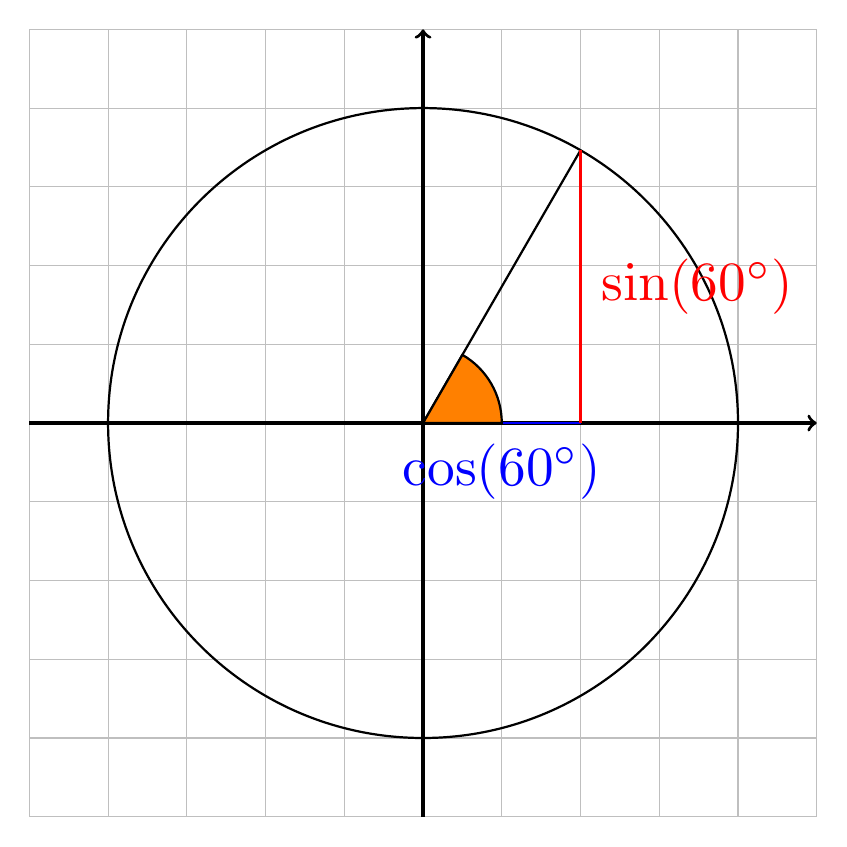
\begin{tikzpicture}[thick,scale=1, every node/.style={scale=2}]

%frid
\draw[lightgray, thin] (-5,-5) grid (5,5);

% axes
\draw[->, very thick] (-5,0) -- (5,0);
\draw[->, very thick] (0,-5) -- (0,5);

% circle
\draw (0,0) circle[radius=4];

% triangle
\draw(0,0) -- (60:4);
\draw[blue] (0,0) -- (2,0);
\draw[red] (2,0) -- (2,4*sin{60});

% lables
\draw[blue] (0,0) -- node[below] {$\cos(60^\circ)$} (2,0);
\draw[red] (2,0) -- node[right] {$\sin(60^\circ)$} (2,4*sin{60});

% angle
\filldraw[fill=orange] (1,0) arc[radius=1, start angle=0, end angle=60] -- (0,0) -- cycle;

\end{tikzpicture}
\end{document}
